\chapter{Results} \label{ch:resultados}

This section provides the main results of the investigation. First, the results reproduced from the original paper \cite{notarmuzi2021percolation} are presented. Then, the results of
the analysis with $n=2$ are shown. Finally, we have studied the behaviour of an inhibitory and excitatory neuron coupled.

\section{Results from the original paper}

The first result is the percolation phase diagram is shown in Figure \ref{f:phase_diagram_article}. It displays the percolation strength $P_{\infty}$ versus the resolution parameter $\Delta$.

\begin{figure}[H]
    \centering
    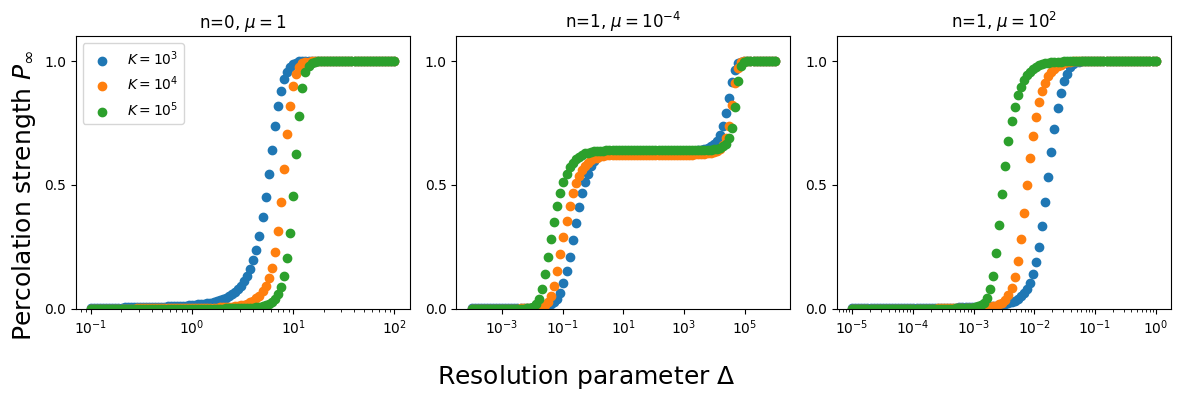
\includegraphics[width=0.95\textwidth]{phase_article_R=1000.png}
    \caption{Percolation phase diagrams for different event number $K$ taking average values of $R=1000$ realizations.}
    \label{f:phase_diagram_article}
\end{figure}

The first plot configuration is a Markovian ($n=0$) Poisson process with rate $\mu$. This is the simplest case, where the inter-event time $x=t_i-t_{i-1}$ follows an exponential 
distribution $P(x_i)=\mu e^{\mu x_i}$. The other two plots are Hawkes processes for $\mu \ll 1$ and $\mu\gg 1$ that are also Markovian as we have chosen an exponential kernel (REFERENCIAR 
AQUÍ A LA PARTE EN LA QUE SE EXPLICA EN METODOLOGÍA.)
. In one hand, a double transition is observed when 
$\mu = 10^{-4}$, in the other hand, a single transition occurs when $\mu = 10^2$. 

Once we have the phase diagram, we can study avalanche statistics. Given a resolution parameter $\Delta$, we can spot clusters or avalanches of activity.
A cluster starts when a neuron fires and ends if the neuron does not fire for a time greater than $\Delta$. We define the size of a cluster as the number of spikes it contains and the duration
as the time between the first and last spike. We have studied the avalanches for $K=10^5$ events and $R=1000$ realizations to obtain the average values since the process is highly not 
stationary. We will study the size and duration of the avalanches for the three different regions of the phase diagram for $\mu=10^{-4}$ and the two regions of the phase diagram for $\mu=10^2$.
These regions are separated by two thresholds, a pseudocritical threshold $\Delta_1^*$ and the threshold of the second transition at $\Delta_2^*$.
We can compute these with the following formulas \cite{notarmuzi2021percolation}:


\begin{align}
    \Delta_1^* &\simeq \dfrac{log(K)}{\langle \lambda \rangle}= \dfrac{log(K)}{\mu+\sqrt{2\mu K}} \label{eq:Ecuación delta1 *} \\
    \Delta_2^* &= \dfrac{log(K)}{\mu}\label{eq:Ecuación delta2 *}
\end{align}

Once we have the thresholds, we can study the avalanches for the different regions of the diagram. The results are shown in Figure \ref{f:avalanches_article}.

\begin{wrapfigure}{l}{0.7\textwidth}
    \begin{center}
      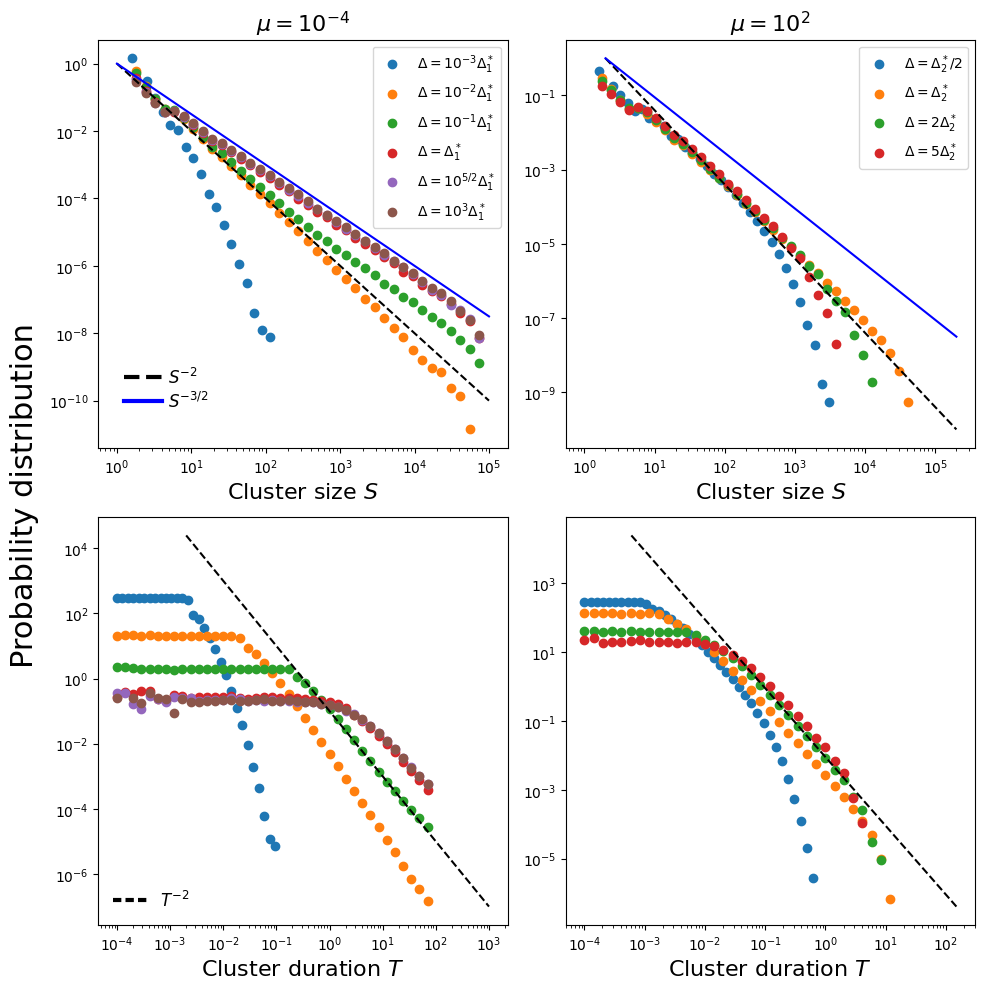
\includegraphics[width=0.675\textwidth]{stats article.png}
    \end{center}
    \caption{Avalanche statistics for a self-exciting Hawkes process with $n=1$ for $K=10^5$ events averaged over $R=1000$ realizations.}
    \label{f:avalanches_article}
\end{wrapfigure}

For $\mu = 10^{-4}$, the results show a power-law distribution for the size and duration of the avalanches
. In the case of duration, the exponent is $\tau=2$ and for the size, we can notice a  
transition of the exponent from $\alpha =2$ to $\alpha =3/2$ as we increase the resolution parameter $\Delta$.
The first exponent corresponds to the universality class of 1D percolation, whereas the second is compatible with the universality class of mean-field branching process.
However, if $\Delta\ll \Delta_1^*$, the behaviour is subcritical for the size and duration of the avalanches.

For $\mu = 10^2$, the result shows another power-law distribution for both size and duration of the avalanches unless $\Delta\ll \Delta_2^*$, where the behaviour is subcritical.
. In this case, the exponents are $\alpha=\tau=2$ corresponding to the universality 
class of 1D percolation.

HABLAR AQUÍ DE LA INFLUENCIA DEL MENOR NÚMERO DE EVENTOS, SE SIGUE PRODUCIENDO LA TRANSICIÓN, PERO PARA OTROS VALORES DE DELTA

\section{Results for n=2}

In the article, the authors have studied a process which is critical itself because the parameter $n$ is fixed to $n=1$. We have studied the case $n=2$ to see if the process is still critical. 
In the Figure \ref{f:n=1 vs n=2} two time series for $n=1$ and $n=2$ are shown. 

\begin{figure}[H]
    \centering
    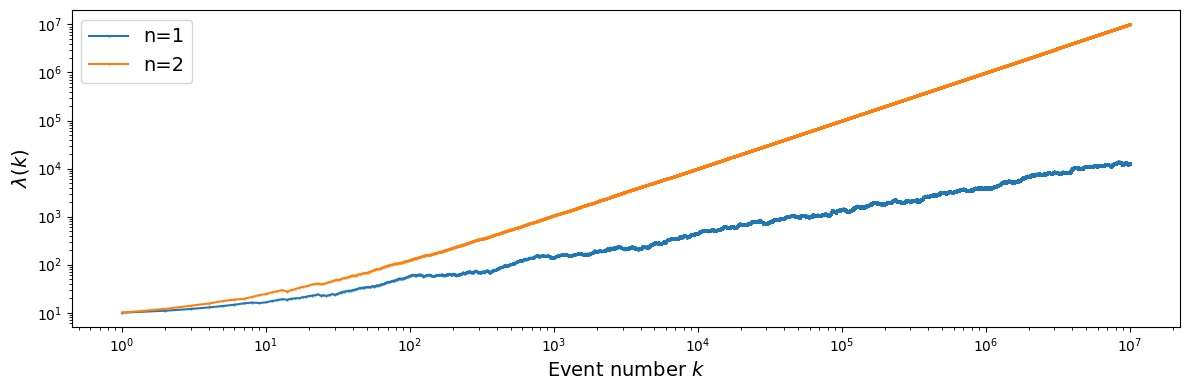
\includegraphics[width=0.65\textwidth]{n=1 vs n=2.png}
    \caption{Time series for $n=1$ and $n=2$.}
    \label{f:n=1 vs n=2}
\end{figure}

Similarly to the previous section, first we obtain the phase diagram in order to observe the transitions. In this case, Eqs \ref{eq:Ecuación delta1 *}-\ref{eq:Ecuación delta2 *} are not valid.
Therefore, we will obtain this parameter graphically from the phase diagrams shown in Figure \ref{f:phase_diagram_n=2}.
\begin{figure}[H]
    \centering
    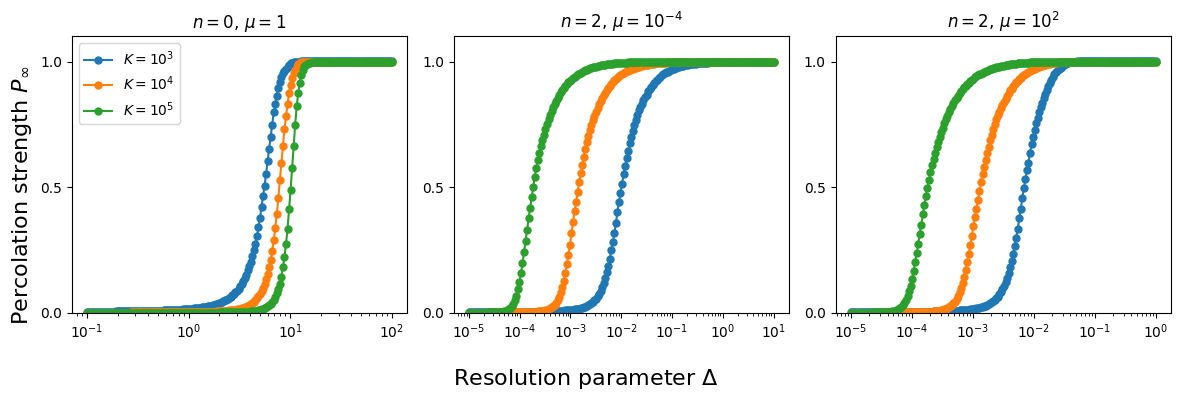
\includegraphics[width=0.95\textwidth]{phase_R=1000_n=2.png}
    \caption{Percolation phase diagrams for a Hawkes process with $n=2$.}
    \label{f:phase_diagram_n=2}
\end{figure}

As we can see, now we have a single transition for $\mu=10^{-4}$ and $\mu=10^2$ corresponding to 1D percolation, consequently, the exponents for the size and duration 
should be $\alpha=\tau=2$. In a similar way, we have studied the avalanches for $K=10^5$ events and $R=1000$ realizations to obtain the average values. The statistics of the avalanches 
are shown in Figure \ref{f:avalanches_n=2}.


\begin{wrapfigure}{l}{0.75\textwidth}
    \begin{center}
      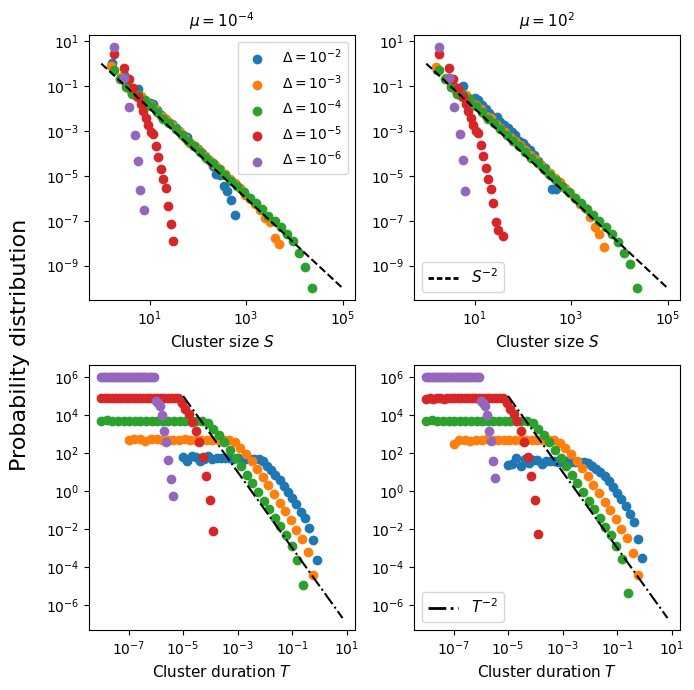
\includegraphics[width=0.675\textwidth]{cutoff_data_dots_n=2.png}
    \end{center}
    \caption{Avalanche statistics for a self-exciting Hawkes process with $n=2$ for $K=10^5$ events averaged over $R=1000$ realizations.}
    \label{f:avalanches_n=2}
\end{wrapfigure}
\clearpage
\section{Inhibitory and excitatory neurons coupled}
